% created by Uwe Schadewald
% modified by Mathias Kuntze and Ahmet Uysal
% Add, handout to documentclass arguments for condensed pdf
\documentclass[presentation, 8pt, mathserif, t]{beamer} % , aspectratio=169
\usepackage[english]{babel}
\usepackage{pgf,graphicx}
\usepackage{amsmath, amssymb}
\usepackage[utf8]{inputenc}
\usepackage{lmodern}
\usepackage{palatino}
\usepackage{multimedia}
\usepackage{pgfpages} 
\usepackage{tikz}
\usepackage{datetime}
\pdfoptionpdfminorversion=5

\usepackage{caption}
\usepackage{subcaption}
% if else
\usepackage{ifthen}
% extend table options
\usepackage{tabularx} 
\usepackage{booktabs}
\usepackage{multicol}
\usepackage{multirow}
\usepackage{eso-pic}  % package to set background image
\usepackage[calc]{picture}

% Packages and stuff for ToDo list like itempoints
\usepackage{pifont}
\newcommand{\cmark}{\ding{51}}%
\newcommand{\xmark}{\ding{55}}%
\newcommand{\open}{$\square$}
\newcommand{\done}{\rlap{$\square$}{\raisebox{1pt}{\large\hspace{1.5pt}\cmark}}\hspace{-2.5pt}}
\newcommand{\wontfix}{\rlap{$\square$}{\raisebox{1pt}{\large\hspace{1.5pt}\xmark}}}
\newcommand{\notsure}{\rlap{$\square$}{\raisebox{0.8pt}{\large\hspace{1.5pt}\textbf{?}}}}



% side bar and footer
\setbeamertemplate{headline}{	
	\leavevmode
	\vspace{-4em}	
	\hbox{		
		\begin{beamercolorbox}[wd=0.85\paperwidth,ht=10ex,dp=8ex,center]{}%			
			% navigation with subsections as dots
			\hspace{3.5em}\insertnavigation{0.7\paperwidth}{\hskip0pt plus1fill} % add navigation in footer						
			% navigation with sections, no subsections
			% \insertsectionnavigationhorizontal{0.6\paperwidth}{\hskip0pt plus1fill}{} \\ % add navigation in footer}
			
		\end{beamercolorbox} 				
	}
	\vskip0pt
}


\setbeamertemplate{footline}{	
	\leavevmode
	\vspace{-3em}
	\hbox{
		\begin{beamercolorbox}[wd=.33\paperwidth,ht=2.25ex,dp=1ex,left]{author in head/foot}%
			\hspace{5em}
			\insertshortauthor
		\end{beamercolorbox}
		\begin{beamercolorbox}[wd=.33\paperwidth,ht=2.25ex,dp=1ex,center]{title in head/foot}%
			\insertshorttitle \ - \insertshortsubtitle
		\end{beamercolorbox}	
		\begin{beamercolorbox}[wd=0.30\paperwidth,ht=10ex,dp=8ex,right]{pagenumber in head/foot}			 	
			\insertframenumber % add page numbers
		\end{beamercolorbox}
	}			
	\vskip0pt
}



\setbeamertemplate{frametitle}{
	\ifthenelse{\equal{\insertframesubtitle}{}}{
		\vspace{0.6cm}
		\huge{\insertframetitle}
	}{
		\vspace{0.6cm}
		\small{\insertframetitle}\\
		\vspace{0.3cm}
		\huge{\insertframesubtitle}
    }		
}

	
% enumerate sections
\setbeamertemplate{section in head/foot}{\hfill\insertsectionheadnumber.~\insertsectionhead}
%\setbeamertemplate{section in head/foot shaded}{\color{structure!50}\hfill\insertsectionheadnumber.~\insertsectionhead}
\setbeamertemplate{section in toc}{\inserttocsectionnumber.~\inserttocsection}

%enumerate subsections
\setbeamertemplate{subsection in head/foot}{\hfill\insertsubsectionheadnumber.~\insertsubsectionhead}
\setbeamertemplate{subsection in head/foot shaded}{\color{structure!50}\hfill\insertsubsectionheadnumber.~\insertsubsectionhead}
%\setbeamertemplate{subsection in toc}[subsections numbered]
\setbeamertemplate{subsection in toc}{\vskip0.5em\leftskip=2em\inserttocsubsection\par}

%--------------------------Common------------------------------------------------------
\setbeamercovered{transparent} % make the beamer theme invisible
\usefonttheme{structurebold}
\beamertemplatenavigationsymbolsempty % set navigations helper function to off
\setbeamertemplate{bibliography item}[text]
\setbeamertemplate{note page}[plain]

%\setlist[itemize,1]{label={$\bullet$}} % \item are using bullets
\setbeamertemplate{itemize items}[circle]
	
	

	
% create a new command to show it on two screens
% I'm using dspdfviewer.
\newcommand{\setDualView} {
	\setbeameroption{show notes on second screen=right}
}

%\AtBeginSection[]{\subsection{}}
\newcommand{\addcite}[1]{%
	\AddToShipoutPictureFG*{%
		\AtPageLowerLeft{%
			\put(0.90\paperwidth,5em){											
				\tiny{
					\cite{#1} 
				}			
			}
		}
	}	
}

% insert a frame with references -> use bibtex
\newcommand{\insertReferenceFrame}[3]{%
	\section{#1}
	\begin{frame}[allowframebreaks]
		\frametitle{#1}
		\bibliographystyle{#2}
		\bibliography{#3}
	\end{frame}	
}

\AtBeginSection[]{\subsection{}}
	





\usepackage{../KU-Beamer-Template/style/koc} 
\usepackage{minted}
\usepackage{upquote}
\usepackage{graphicx}

% pdflatex --shell-escape lecture5.tex & pdflatex --shell-escape lecture5.tex

\title{KOLT Python}
\subtitle{Functions} 
\newdate{date}{25}{02}{2020}
\date{\displaydate{date}}
\author{Ahmet Uysal}

\titlegraphic{
\includegraphics[scale=0.18]{../KU-Beamer-Template/style/images/kolt_logo.png}}

\setbeamercovered{invisible} % transparent
\makeatletter
\let\@@magyar@captionfix\relax
\makeatother
\begin{document}
    \maketitle

    \frame{\frametitle{Agenda}\tableofcontents}
    
    \section{Recap}

    \subsection{Loops}

    \begin{frame}{\texttt{while} \& \texttt{for} Loops}
        \begin{columns}
            \begin{column}{0.45\textwidth}
                \inputminted[frame=single,framesep=2pt]{python3}{../Lecture3/code-examples/while1.py}
                \pause
                Repeat some \texttt{<expression>}s \underline{as long as} a \texttt{<condition>} is \texttt{True}.
                \pause
                \medskip
                \texttt{<condition>} is only checked \textbf{\underline{before}} each execution.
            \end{column}
            \pause
            \begin{column}{0.45\textwidth}
                \inputminted[frame=single,framesep=2pt]{python3}{../Lecture3/code-examples/for1.py}
                \pause
                Repeat some \texttt{<expression>}s for \textbf{each} element of a \texttt{<iterable>}.
            \end{column} 
        \end{columns}
    \end{frame}

    \begin{frame}{\texttt{break} \& \texttt{continue} statements}
        \Large
        \texttt{break} \& \texttt{continue} statements can alter the \textbf{normal flow} of a loop.\\
        \pause
        \LARGE
        \texttt{\textbf{break}}:
        \begin{itemize}
            \pause
            \item Immediately terminates the loop
        \end{itemize}
        \pause
        \texttt{\textbf{continue}}:
        \pause
        \begin{itemize}
            \item Jumps to the \textbf{next iteration} of the loop
            \pause
            \begin{itemize}
                \large
                \item \texttt{while}: \pause jump to the control step \pause
                \item \texttt{for}: \pause jump to the next element of a the \texttt{<iterable>}.
            \end{itemize}
        \end{itemize}
    \end{frame}

    \subsection{Lists}

        \begin{frame}{Lists}
            \begin{center}
                
\includegraphics[width=0.6\textwidth]{../Lecture1/images/box_many.jpg}                
            \end{center}
            \LARGE
            Imagine variables, but with limitless capacity$\dots$\\
            \textbf{\texttt{sunnyside = [\textquotesingle Mr. Potato Head\textquotesingle, \textquotesingle Hamm\textquotesingle,
            \textquotesingle Buzz Lightyear\textquotesingle, \textquotesingle Slinky Dog\textquotesingle]}}
        \end{frame}

        \begin{frame}{List Operations}
            \Large
            \textbf{\texttt{list.append(x)}}: Append x to end of the sequence\\
            \textbf{\texttt{list.insert(i, x)}}: Insert x to index i\\
            \textbf{\texttt{list.pop(i=-1)}}: Remove and return element at index i\\
            \textbf{\texttt{list.remove(x)}}: Remove first occurrence of x\\
            \textbf{\texttt{list.extend(iterable)}}: Add all elements in iterable to end of list\\
            \textbf{\texttt{list[i] = new\_value}}: Update value of index i with new value\\
            \textbf{\texttt{list[basic\_slice] = iterable}}: Change elements in basic slice with elements in iterable, sizes can be different: \texttt{numbers[:] = []}\\
            \textbf{\texttt{list[extended\_slice] = iterable}}: Change elements in extended slice with elements in iterable 1-1, sizes must be equal.\\
        \end{frame}

        \begin{frame}{List Operations (cont.)}
            \Large
            \textbf{\texttt{in}} operator: Check whether an element is in list.\\
            \texttt{3 in numbers} $\Rightarrow$ \texttt{True}\\
            \textbf{\texttt{len(list)}}: Returns the length of list(and other collections).\\
            \textbf{\texttt{list.index(value, start=0, stop=len(list))}}:\\
            Return first index of value.\\
            \textbf{\texttt{list.count(value)}}: Count number of occurrences of value.\\
            \textbf{\texttt{list.reverse()}}: Reverse the list (in-place)\\
            \textbf{\texttt{list.sort()}}: Sort list elements (in-place)\\
            \\ 
            For more, type \texttt{help(list)} in your interactive interpreter.
        \end{frame}

    \subsection{Basic Functions}

    \begin{frame}[c]{Functions}
        \LARGE
        Functions are blocks of
        \pause
        \textbf{organized},
        \pause
        \textbf{reusable} code
        \pause that carry some \textbf{specific} tasks.\\
        \pause
        \begin{center}
            
\includegraphics[width=0.3\textwidth]{../Lecture2/images/reduce_reuse_recycle.png}
        \end{center}
    \end{frame}

    \begin{frame}{Defining Functions}
        \LARGE
        \textbf{\texttt{def}} keyword introduces a function \textbf{\textit{definition}}.
        \\
        \large
        \inputminted[firstline=14, lastline=16, frame=single,framesep=2pt]{python3}{../Lecture2/code-examples/menemen.py}
        \inputminted[firstline=18, lastline=20, frame=single,framesep=2pt]{python3}{../Lecture2/code-examples/menemen.py}
    \end{frame}

    \subsubsection{Exercise}

    \begin{frame}{Exercise}
        \Large
        Assume we have a list that contains scores of all football matches that are played between Fenerbahçe and Galatasaray at Şükrü Saraçoğlu Stadium.\\
        \pause
        \texttt{scores = [[5, 1], $\dots$, [1, 3]]}\\\pause
        For both teams, we want to find:\\\pause
        \begin{enumerate}
            \item Longest unbeaten runs \pause
            \item Longest winning streaks \pause
            \item Number of matches to last win \pause
        \end{enumerate}

        \href{https://github.com/koltpython/python-slides/raw/master/Lecture5/code-examples/rivalry.py}{\underline{\textit{Starter Code}}}
        
    \end{frame}

    \section{Functions}
        \subsection{Defining Functions}
        \begin{frame}{Functions}
            \pause
            \LARGE
            Functions are blocks of \textbf{organized}, \textbf{reusable} code that carry some \textbf{specific} tasks.
            \pause
            \begin{itemize}
                \item \textbf{\texttt{input([prompt])}:} \\
                \pause
                If the prompt \textbf<5->{argument} is present, it is written to standard output without a trailing newline. The function then reads a line from input, converts it to a string (stripping a trailing newline), and \textbf<5->{returns} that. When \texttt{EOF} is read, \texttt{EOFError} is \textbf<5->{raised}.   
            \end{itemize}

            \pause
            \pause

            \begin{center}
                \tikzstyle{int}=[draw, fill=blue!20, minimum size=2em]

                \begin{tikzpicture}[node distance=2.5cm,auto]
                    \node [int] (a) {$function$};
                    \node (b) [left of=a,node distance=4cm, coordinate] {a};
                    \node [coordinate] (end) [right of=a, node distance=4cm]{};
                    \path[->] (b) edge node {$*arguments$} (a);
                    \draw[->] (a) edge node {\texttt{return}} (end) ;
                \end{tikzpicture}
            \end{center}
        \end{frame}   
 
        \begin{frame}{Defining Functions}
            \pause
            \LARGE
            \textbf{\texttt{def}} keyword introduces a function \textit{definition}.
            \normalsize
            \pause
            \inputminted[frame=single,framesep=2pt, lastline=8]{python3}{code-examples/function_def.py}
            \pause
            \inputminted[frame=single,framesep=2pt, lastline=8]{python3}{code-examples/function_def2.py}
            \pause
            \inputminted[frame=single,framesep=2pt, lastline=8]{python3}{code-examples/function_def3.py}
        \end{frame}


        \begin{frame}{Functions}
            \inputminted[frame=single,framesep=2pt]{python3}{code-examples/function_ex.py}
            \pause
            \inputminted[frame=single,framesep=2pt]{python3}{code-examples/function_ex2.py}
        \end{frame}

        \begin{frame}{Functions}
            \LARGE
            \textit{Defining} a \texttt{function} only makes it available.\\
            \pause 
            You should \textit{call} the \texttt{function} to execute.\\           
            \pause
            \newline
            \textbf{\texttt{fib\_100 = fibonacci\_series(100)}}\\
            \pause
            \textbf{\texttt{what\_is\_going\_on = print(fib\_100)}}\\
            \newline
        \end{frame}

      \subsection{return Statement}

        \begin{frame}{return Statement}
            \LARGE
            \pause
            \inputminted[frame=single,framesep=2pt]{python3}{code-examples/return.py}
            \pause
            Return \textbf{immediately} terminates the function.\\
            So, \texttt{print(\textquotesingle Doubled\textquotesingle)} is not executed by Python.
        \end{frame}

        \begin{frame}{return Statement}
            \LARGE
            \visible<2->{\textbf{Every} function returns \textbf{one} value!} 
            \newline
            \visible<4->{\texttt{value = }}\visible<3->{\texttt{\textbf{print}(\textquotesingle Hello, World!\textquotesingle )}}
            \newline
            \visible<5->{\texttt{\textbf{print}(value)}}
            \newline
            \visible<6->{Functions implicitly return \texttt{None} if they complete without a return statement.}
        \end{frame}

        \begin{frame}{Example Revisited}
            \LARGE
            \pause
            \texttt{\textbf{def} largest\_unbeaten\_run(team\_name):}\\ \pause
            \texttt{\textbf{def} largest\_winning\_streak(team\_name):}\\ \pause
            \texttt{\textbf{def} matches\_to\_last\_win(team\_name):}\\ 
        \end{frame}

      \subsection{Parameters}    
        \begin{frame}{Default Parameters}
            The values of parameters can be set to used as default.
            \newline
            In \textbf{\texttt{print(*args, sep=\textquotesingle \ \textquotesingle, end=\textquotesingle \textbackslash n\textquotesingle )}}, 
            sep and end has default values.
            \pause
            \inputminted[frame=single,framesep=2pt, lastline=15]{python3}{code-examples/default.py}
            \textbf{Valid Uses}
            \begin{columns}
                \begin{column}{0.50\textwidth}
                    \pause
                    \inputminted[frame=single,framesep=2pt, lastline=15]{python3}{code-examples/valid1.py}  
                \end{column}
                \begin{column}{0.50\textwidth}
                    \pause
                    \inputminted[frame=single,framesep=2pt, lastline=15]{python3}{code-examples/valid1_1.py}                    
                \end{column}
            \end{columns}
        \end{frame}

        \begin{frame}{Default Parameters}
            \inputminted[frame=single,framesep=2pt, lastline=15]{python3}{code-examples/default.py}
            \pause
            \LARGE
            \textbf{Invalid Usages}
            \inputminted[frame=single,framesep=2pt, lastline=15]{python3}{code-examples/valid2.py}  
        \end{frame}

        \begin{frame}{Example Revisited}
            \LARGE
            How can we make our functions return results for Galatasaray by default?\\ \pause
            \texttt{\textbf{def} largest\_unbeaten\_run(team\_name\pause =\textquotesingle GS\textquotesingle):}\\ \pause
            \texttt{\textbf{def} largest\_winning\_streak(team\_name=\textquotesingle GS\textquotesingle):}\\ \pause
            \texttt{\textbf{def} matches\_to\_last\_win(team\_name=\textquotesingle GS\textquotesingle):}\\
        \end{frame}

        \begin{frame}{Variadic Positional Arguments}
            \pause
            \LARGE
            Can functions accept arbitrary number of arguments?
            \newline
            In \textbf{\texttt{print(*args, sep=\textquotesingle \ \textquotesingle, end=\textquotesingle \textbackslash n\textquotesingle )}}, 
            you can put as many args as you want.
            \pause
            \newline 
            \newline Suppose we want a \texttt{max} function that works as so:
            \newline max(3, 5) gives 5.
            \newline max(3, 4, 2) gives 4.
            \newline product(3, 5, -1, 2, 10, 20, 13, 34) gives 34.
            \newline 
        \end{frame}

        \begin{frame}{Variadic Positional Arguments: my\_max}
          \pause
          \large
          \inputminted[frame=single,framesep=2pt]{python3}{code-examples/variadic.py}
        \end{frame}

        \begin{frame}{Announcements}
            \LARGE
            Fill out the attendance form:\\
            \href{https://tiny.cc/koltpython}{\underline{\textit{tiny.cc/koltpython}}}\\
            Keyword: \textbf{functions}\\
            \pause
            Assignment I: Tic-Tac-Toe is posted!
            
            \begin{center}
                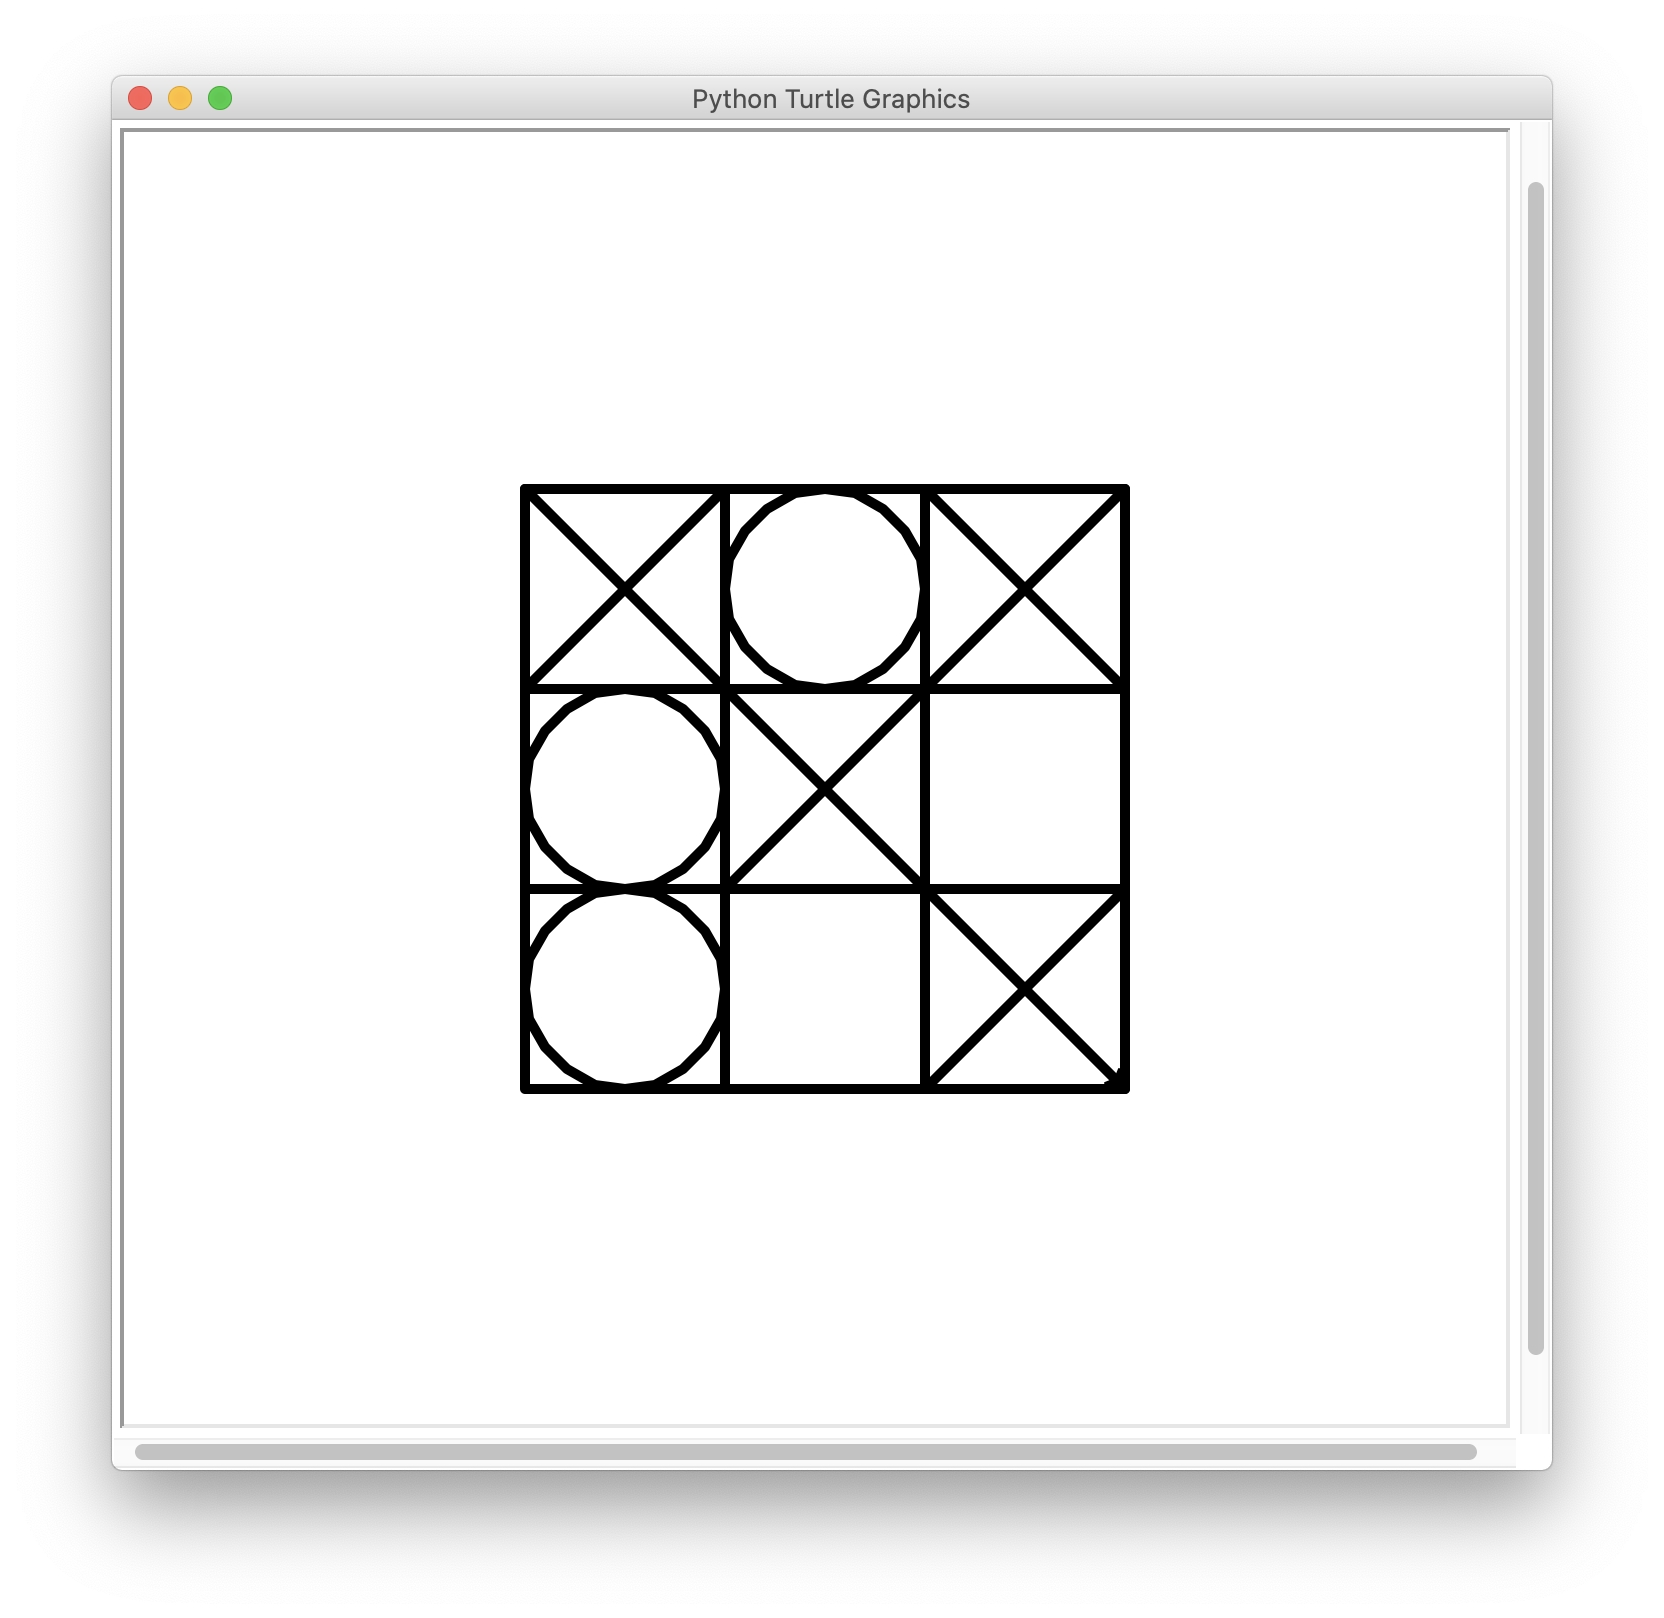
\includegraphics[width=0.3\textwidth]{images/end_game_figure.png}
            \end{center}
        
        \end{frame}
\end{document}